\documentclass[a4paper]{article}

\usepackage{html}
\usepackage{hthtml}
\usepackage{xspace}
\usepackage{url}
\usepackage{graphicx}

\newcommand{\Jason}[0]{\htlink{\textit{Jason}}{http://jason.sf.net}\xspace}


\begin{document}

\html{
\begin{rawhtml}
  <div class=title>Interoperation between <b><i>Jason</i></b> and JADE Multi-Agent
  Systems</div>
\end{rawhtml}}

This document aims to show how to create \Jason agents that
participate in an multi-agent system (MAS) formed by ``normal'' JADE
agents (by normal we mean being not developed considering
interoperability with \Jason, i.e., any existing JADE agent). We will
develop a \Jason book-seller agent that joints the system of the
traditional example of book trading that comes with JADE. The JADE
code will remain as in the example, it will not be changed to
interoperate with \Jason.

\tableofcontents

\section{Accessing the JADE DF from \Jason}

The first thing a seller agent should do is to register itself as a
book seller in the JADE DF (Directory Facilitator) service. The
standard AgentSpeak language does not have a command for this purpose,
of course; however, in \Jason, we can create a new internal action in
Java that can do the job.

The following steps create a new \Jason project for our seller agent
and an internal action that register it in JADE's DF:

\begin{enumerate}
\item Create a new project called ``book_trading'' that uses Jade as
  the infrastructure.
  
  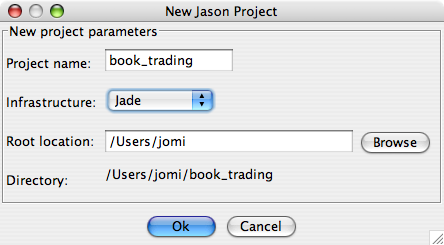
\includegraphics{figures/screen-create-project.png}

\item Create the first version of the seller agent, called
  \texttt{john}, with the following code:

\begin{verbatim}
// Agent john in project book_trading.mas2j

/* Initial beliefs and rules */

// A 'book' belief has three arguments:
//   . the title
//   . its price
//   . the quantity in stock

book("Harry", 32, 20).
book("Jason", 50, 10).


/* Initial goals */

!registerDF.

/* Plans */

+!registerDF <- jadedf.register("book-selling","JADE-book-trading").
\end{verbatim}

  The \texttt{jadedf.register("book-selling","JADE-book-trading")}
  code calls the internal action named \texttt{register} in a package
  called \texttt{jadedf}.

\item To create this internal action, click on
  the \includegraphics{figures/createIA.gif} ican and fill in the form
  as follows:

  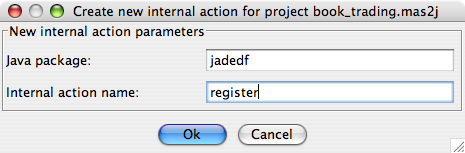
\includegraphics{figures/screen-create-ia.png}

  The source code of this internal action is as follows (the
  \texttt{execute} method has the code for the internal action and
  \texttt{args} contains the arguments given in the AgentSpeak code):

\begin{verbatim}
package jadedf;

import jade.domain.*;
import jade.domain.FIPAAgentManagement.*;
import jason.asSemantics.*;
import jason.asSyntax.*;
import jason.infra.jade.JadeAgArch;

import java.util.logging.Logger;

/** 
 * Register a service in the jade DF (available only when the JADE infrastructure is used)
 *
 * This internal action does not replace the services of the agent but
rather adds a new service.
 *
 * The first argument is the service type and
 * the second is the name (they should be of type String).
 * 
 * @author Jomi
 */
public class register extends DefaultInternalAction {

    private Logger logger = Logger.getLogger("JadeDF.mas2j."+register.class.getName());

    @Override
    public Object execute(TransitionSystem ts, Unifier un, Term[] args) throws Exception {
        try {
            if (ts.getUserAgArch().getArchInfraTier() instanceof JadeAgArch) {
                // get a reference to the JADE agent that represents this Jason agent
                JadeAgArch infra = (JadeAgArch)ts.getUserAgArch().getArchInfraTier();

                // 0. get arguments from the AgentSpeak code (type and name of the new service)
                StringTerm type = (StringTerm)args[0];
                StringTerm name = (StringTerm)args[1];
                
                // 1. get current services
                DFAgentDescription dfd = new DFAgentDescription();
                dfd.setName(infra.getAID());

                DFAgentDescription list[] = DFService.search( infra, dfd );

                // 2. deregister
                if ( list.length > 0 ) { 
                    DFService.deregister(infra);
                    dfd = list[0]; // the first result 
                }

                // 3. add a new services
                ServiceDescription sd = new ServiceDescription();
                sd.setType(type.getString());
                sd.setName(name.getString());
                dfd.addServices(sd);
                
                // 4. register again
                DFService.register(infra, dfd);
                
                return true;
            } else {
                logger.warning("jadefd.register can be used only with JADE infrastructure.");
            }
        } catch (Exception e) {
            logger.warning("Error in internal action 'jadedf.register'! "+e);
        }
        return false;
    }
}
\end{verbatim}


\item You can now run the project and use the menu option ``Tools ->
  Show DF'' of the RMA agent to inspect the DF:

 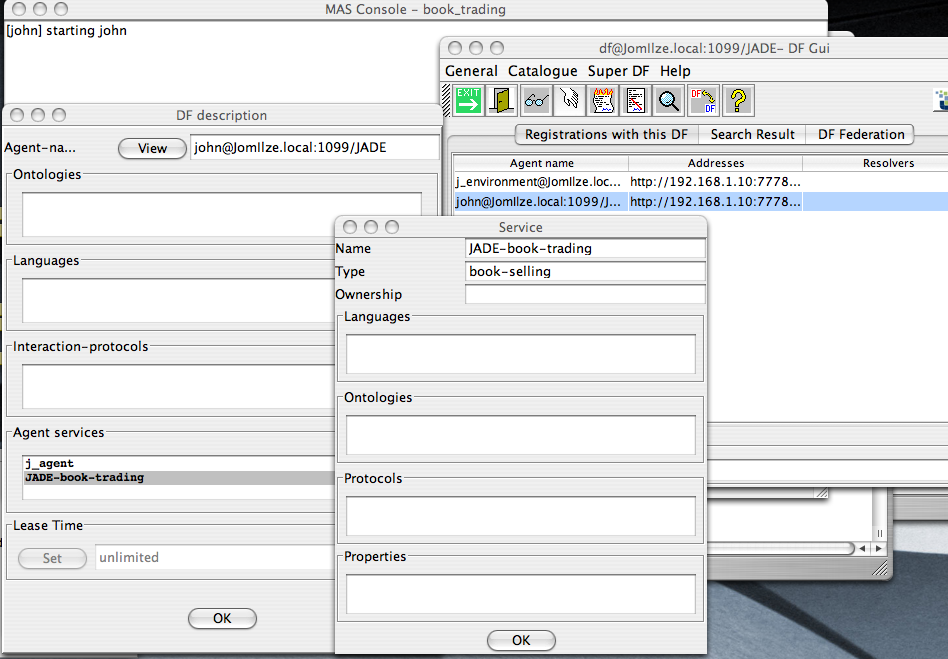
\includegraphics{figures/screen-df.png}

\end{enumerate}



\section{Creating a seller in \Jason}

The buyer agent, written in JADE, retrieves information about all
sellers from the DF, and then sends a CFP (call for proposal) message
to all those agents. Since \Jason agents use KQML-like performatives,
the performatives used by JADE agents are not available in \Jason,
i.e., the semantics of those performatives are not implemented in
\Jason (which implements the semantics of performatives such as tell,
askOne, achieve, etc.). We need therefore to write ``low level'' plans
to handle in AgentSpeak the CFP messages from JADE agents.

Every message that arrives in to \Jason agent (and is accepted for
processing) produces an event like \texttt{+!kqml_received(Sender,
  Performative, Content, MsgId)} (the MsgId should be used to reply to
the message). We can then create plans to handle this event in the
particular case where the performative is CFP or ACCEPT_PROPOSAL:

\begin{verbatim}
// Agent john in project book_trading.mas2j

/* Initial beliefs and rules */

// The book beliefs has three arguments:
//   . the book name
//   . the price
//   . the quantity in stock

book("Harry", 32, 20).
book("Jason", 75, 10).


/* Initial goals */

!registerDF.

/* Plans */

+!registerDF <- jadedf.register("book-selling","JADE-book-trading").


/* handle CFP performatives */

// CFP
+!kqml_received(Sender, cfp, Content, MsgId)
  :  book(Content, Price, Qtd) & Qtd > 0            // if I have the book,
  <- .send(Sender, propose, Price, MsgId).          // propose;
  
+!kqml_received(Sender, cfp, Content, MsgId)
  <- .send(Sender, refuse, "not-available", MsgId). // otherwise, refuse.

  
// ACCEPT-PROPOSAL	 
+!kqml_received(Sender, accept_proposal, Content, MsgId)
  :  book(Content, Price, Qtd) & Qtd > 0  // If I still have the book
  <- -+book(Content, Price, Qtd-1);       // change stock
     .print("New stock for ", Content, " is ", Qtd-1);
     .send(Sender, tell, Content, MsgId). // confirm 

+!kqml_received(Sender, accept_proposal, Content, MsgId)
  <- .send(Sender, failure, "not-available", MsgId).
\end{verbatim}

\section{Running the system}

Follow the steps below to run the system with JADE and \Jason agents:

\begin{enumerate}
\item \Jason 1.0 does not allow the use of FIPA-ACL performatives,
  so replace the Jason/lib/jason.jar file by the one available
  \htlink{here}{jason.jar}.

\item Start the JADE main container and the seller agent using the
  
\includegraphics{figures/run.png} button in jEdit.

\item Download the buyer agent from
  \htlink{here}{../../getting-started-jade/html/jade-example.zip}. (It
  is the one used in the \htlink{JADE
    exercise}{../../getting-started-jade/html/index.html}.)


\item Start the buyer, called \texttt{bob}, in a new container using
  the command
\begin{verbatim}
jade.Boot -container -host localhost bob:examples.bookTrading.BookBuyerAgent(Harry)
\end{verbatim}

It will try to buy a book entitled ``Harry''.

The output from the buyer is:
\begin{verbatim}
Hallo! Buyer-agent bob@JomIlze.local:1099/JADE is ready.
Target book is Harry
Trying to buy Harry
Found the following seller agents:
john@JomIlze.local:1099/JADE
Harry successfully purchased from agent john@JomIlze.local:1099/JADE
Price = 32
Buyer-agent bob@JomIlze.local:1099/JADE terminating.
\end{verbatim}
\end{enumerate}


You can also run the whole system without jEdit:
\begin{enumerate}
\item First start the buyer in the main container:
\begin{verbatim}
jade.Boot -gui "bob:examples.bookTrading.BookBuyerAgent(Harry)"

\end{verbatim}
\item Start the \Jason seller as follows (ensure that all JADE jars
  are in the CLASSPATH):
\begin{verbatim}
cd <directory where the book_trading example was saved>
export CLASSPATH=$CLASSPATH:bin/classes
java jade.Boot -container -host localhost "john:jason.infra.jade.JadeAgArch(john.asl)"
\end{verbatim}
\end{enumerate}

\section{Exercises}

\begin{enumerate}
\item Run the agents in different machines.
\item Write the code for a buyer agent in \Jason that uses the DF to
  find sellers, sends a CFP, select the cheapest, and only then buys
  the book.
\end{enumerate}

\end{document}


